% Minkowski-Diagramm: Achsen von S' (beta = 0.5), Lichtkegel, Eichhyperbeln, Gleichzeitigkeit
% Gemeinsamer Stil für alle Abbildungen (TikZ -> SVG, siehe figures/build.mjs).
%
% Farben sind Platzhalter ("Sentinels"): build.mjs ersetzt sie im SVG durch
% CSS-Variablen, damit die Abbildungen im hellen und dunklen Modus passen.
% Andere Farben (auch schwarz/weiß) bricht der Build mit Fehler ab.
%
%   fg    Linien, Beschriftung          -> --dark
%   mu    Hilfslinien, Achsen, Maße      -> --gray
%   acc   das eine Konzept der Abbildung -> --secondary (Lime/Oliv)
%   blue  zweite Größe, negative Ladung  -> --fig-blue
%   warm  dritte Größe, positive Ladung  -> --fig-warm
%   bg    Seitenhintergrund (Aussparen)  -> --light
%
% Kein \clip verwenden: pdftocairo macht daraus Clip-Gruppen, in denen exakt
% waagerechte/senkrechte Linien verschwinden. Berechnete Kurven schneidet
% gen/*.py selbst am Rahmen ab.
\documentclass[tikz,border=3pt]{standalone}
\usepackage{amsmath,amssymb,bm}
% Text serifenlos wie die Seite, Mathe in Computer Modern wie KaTeX
\renewcommand{\familydefault}{\sfdefault}
\usetikzlibrary{arrows.meta,calc,decorations.markings,patterns,3d,positioning,angles,quotes}

\definecolor{fg}{RGB}{1,2,3}
\definecolor{mu}{RGB}{4,5,6}
\definecolor{acc}{RGB}{7,8,9}
\definecolor{blue}{RGB}{10,11,12}
\definecolor{warm}{RGB}{13,14,15}
\definecolor{bg}{RGB}{16,17,18}

% Vektoren wie auf der Website (KaTeX \mathbf)
\newcommand{\vv}[1]{\mathbf{#1}}

\tikzset{
  every picture/.style={fg, line width=0.8pt, line cap=round, line join=round,
    >={Stealth[length=5.5pt,width=4.4pt]}},
  every node/.style={font=\small},
  % Linientypen
  main/.style={line width=0.9pt},
  thin/.style={line width=0.5pt},
  aux/.style={mu, line width=0.5pt, dash pattern=on 2.5pt off 2pt},
  axis/.style={mu, line width=0.6pt, ->},
  vec/.style={line width=1.1pt, ->},
  field/.style={line width=0.7pt, postaction={decorate},
    decoration={markings, mark=at position #1 with {\arrow{Stealth[length=4.5pt,width=3.6pt]}}}},
  field/.default=0.5,
  % Flächen
  soft/.style={fill=#1, fill opacity=0.14},
  soft/.default=acc,
  % Ladungen
  qpos/.style={circle, fill=warm, inner sep=0pt, minimum size=9pt,
    path picture={\draw[bg, line width=0.9pt] ($(path picture bounding box.center)+(-2pt,0)$) -- +(4pt,0)
      ($(path picture bounding box.center)+(0,-2pt)$) -- +(0,4pt);}},
  qneg/.style={circle, fill=blue, inner sep=0pt, minimum size=9pt,
    path picture={\draw[bg, line width=0.9pt] ($(path picture bounding box.center)+(-2pt,0)$) -- +(4pt,0);}},
  dot/.style={circle, fill=fg, inner sep=0pt, minimum size=3pt},
  % Beschriftung mit Aussparung, damit Linien den Text nicht kreuzen
  lbl/.style={fill=bg, inner sep=1.5pt},
  % Icons: kräftigere Linien, keine Schrift
  icon/.style={line width=1.6pt, >={Stealth[length=6pt,width=5pt]}},
}

\begin{document}
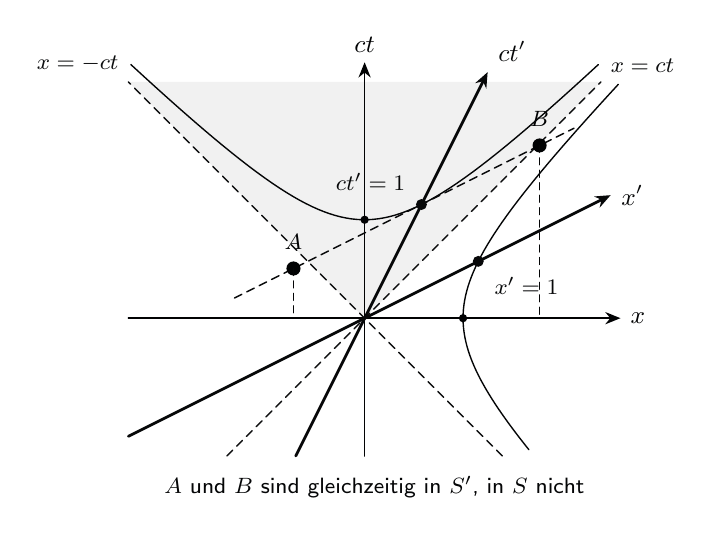
\begin{tikzpicture}[scale=1.25]
  \def\b{0.5}
  \pgfmathsetmacro{\g}{1/sqrt(1-\b*\b)}
  % Lichtkegel
  \fill[warm, fill opacity=0.06] (0,0) -- (2.4,2.4) -- (-2.4,2.4) -- cycle;
  \draw[warm, thin, dash pattern=on 3pt off 2pt] (-1.4,-1.4) -- (2.4,2.4) node[anchor=south west, font=\footnotesize] {$x=ct$};
  \draw[warm, thin, dash pattern=on 3pt off 2pt] (1.4,-1.4) -- (-2.4,2.4) node[anchor=south east, font=\footnotesize] {$x=-ct$};
  % Eichhyperbeln (ct)^2 - x^2 = 1 und x^2 - (ct)^2 = 1
  \draw[mu, thin, domain=-1.6:1.6, samples=60, variable=\t] plot ({sinh(\t)},{cosh(\t)});
  \draw[mu, thin, domain=-1.1:1.6, samples=60, variable=\t] plot ({cosh(\t)},{sinh(\t)});
  % Achsen S
  \draw[axis, fg] (-2.4,0) -- (2.6,0) node[anchor=west] {$x$};
  \draw[axis, fg] (0,-1.4) -- (0,2.6) node[anchor=south] {$ct$};
  % Achsen S': ct'-Achse x = beta ct, x'-Achse ct = beta x
  \draw[acc, line width=1pt, ->] (-1.4*\b,-1.4) -- (2.5*\b,2.5) node[anchor=south west] {$ct'$};
  \draw[acc, line width=1pt, ->] (-2.4,-2.4*\b) -- (2.5,2.5*\b) node[anchor=west] {$x'$};
  % Einheiten auf den gestrichenen Achsen (Schnitt mit den Hyperbeln)
  \node[acc, circle, fill=acc, inner sep=1.4pt] at ({\g*\b},{\g}) {};
  \node[acc, circle, fill=acc, inner sep=1.4pt] at ({\g},{\g*\b}) {};
  \node[acc, font=\footnotesize, anchor=south east] at ({\g*\b-0.06},{\g+0.04}) {$ct'=1$};
  \node[acc, font=\footnotesize, anchor=north west] at ({\g+0.06},{\g*\b-0.06}) {$x'=1$};
  % Einheiten in S
  \node[dot] at (0,1) {}; \node[dot] at (1,0) {};
  % Gleichzeitigkeit in S': Linie parallel zur x'-Achse durch ct'=1
  \draw[acc, thin, dash pattern=on 3pt off 2pt] ({\g*\b-1.9},{\g-1.9*\b}) -- ({\g*\b+1.55},{\g+1.55*\b});
  \coordinate (A) at ({\g*\b-1.3},{\g-1.3*\b});
  \coordinate (B) at ({\g*\b+1.2},{\g+1.2*\b});
  \node[circle, fill=fg, inner sep=1.8pt, label={[font=\footnotesize]above:$A$}] at (A) {};
  \node[circle, fill=fg, inner sep=1.8pt, label={[font=\footnotesize]above:$B$}] at (B) {};
  \draw[aux] (A) -- (A |- 0,0);
  \draw[aux] (B) -- (B |- 0,0);
  \node[mu, font=\footnotesize, align=center, anchor=north] at (0.1,-1.5) {$A$ und $B$ sind gleichzeitig in $S'$, in $S$ nicht};
\end{tikzpicture}
\end{document}
